\documentclass{article}[12pt]
\usepackage[utf8]{inputenc}
\usepackage[T1]{fontenc}
\usepackage{array}
\usepackage{eqnarray}
\usepackage{caption}
\usepackage{amsmath}
\usepackage[toc,page]{appendix}
\usepackage{amssymb}
\usepackage{comment}
\usepackage{hyperref}
\usepackage{fancybox}
\usepackage{gensymb}
\usepackage[english]{babel}
\usepackage{graphicx}
\usepackage{subcaption}
\usepackage{wrapfig}
\usepackage{xcolor}
\usepackage{mdframed}
\usepackage{titlepic}
\usepackage{titling}
\usepackage{listings}
\usepackage{placeins}
\usepackage{multicol}
\usepackage{authblk}
\usepackage{geometry}
\usepackage{float}
\geometry{hmargin=2.5cm,vmargin=2cm}
\usepackage{listings}
\usepackage{textcomp}
\usepackage{gensymb}
\usepackage{natbib}
\definecolor{codegreen}{rgb}{0,0.6,0}
\definecolor{codegray}{rgb}{0.5,0.5,0.5}
\definecolor{codepurple}{rgb}{0.58,0,0.82}
\definecolor{backcolour}{rgb}{0.95,0.95,0.92}
\hypersetup{
    colorlinks,
    linkcolor={blue!10!black},
    citecolor={blue!50!black},
    urlcolor={blue!50!black}
}
\usepackage{array,multirow,makecell}
\setcellgapes{1pt}
\makegapedcells
\newcolumntype{R}[1]{>{\raggedleft\arraybackslash }b{#1}}
\newcolumntype{L}[1]{>{\raggedright\arraybackslash }b{#1}}
\newcolumntype{C}[1]{>{\centering\arraybackslash }b{#1}}

\title{Electronic for measurement systems - Weighing scale}
\author{Pierre-Louis GIL and Youwan MAHÉ}
\date{Nov-Dec 2022, Grenoble-INP PHELMA}

\begin{document}

\maketitle
\tableofcontents
\newpage

\section{Sensor}
\paragraph{}
The main component behind weighing scales is the \emph{Straining Gauge}. Straining gauges are resistive sensors that are used to measure strain on an object. The resistive part is usually made of metal and glued to an insulating adhesive surface such as cyanoacrylate. Since the variation of resistance is  small, it is very common to use a Wheatstone bridge configuration to transform the variation of resistance in a differential voltage \cite{LeBerre-2016}.
\subsection{Gauge factor and measurand}
\paragraph{}
The Gauge Factor $GF$ is a quantity used to describe the sensitivity of a strain gauge. \cite{bucci}
\begin{equation}
GF=\dfrac{\Delta R/R}{\epsilon}
\end{equation}
\begin{itemize}
\item $\epsilon$ is the strain (ration between length under stress and length at rest)
\item $\Delta R$ The variation of resistance
\item $R$ Resistance at rest
\end{itemize}
Using the Wheatstone bridge, we convert the $\Delta R$ in a differential voltage $V_{sensor}$.
\begin{figure}[H]
\centering
\begin{subfigure}{.5\textwidth}
  \centering
  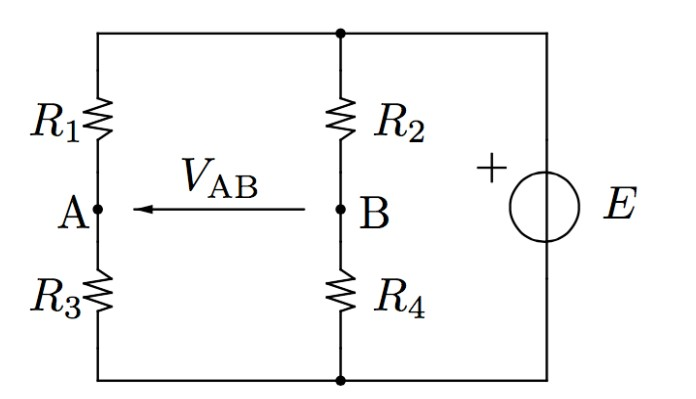
\includegraphics[width=.8\linewidth]{figures/wheatstone.jpg}
  \caption{Wheatstone's bridge schematic}
  \label{fig:Wheatstone}
\end{subfigure}%
\begin{subfigure}{.5\textwidth}
  \centering
  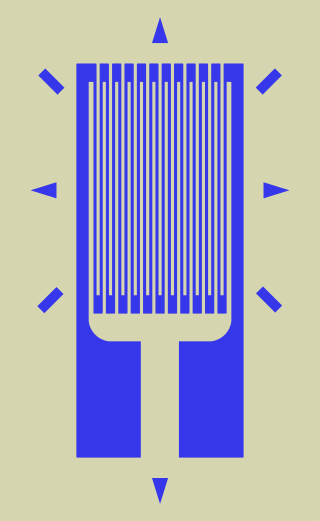
\includegraphics[width=.4\linewidth]{figures/Strain_gauge.png}
  \caption{Staining gauge \cite{LeBerre-2016}}
  \label{fig:sub2}
\end{subfigure}
\caption{}
\label{fig:test}
\end{figure}
\begin{equation}
V_{sensor}=\dfrac{GF \epsilon}{4}E
\end{equation}
\begin{itemize}
\item $E$ is the bridge voltage at rest
\item $GF$ the gauge factor
\item $\epsilon$ The strain
\item $V_{sensor}$ the differential voltage
\end{itemize}
\paragraph{}
Our strain gauge is the model DF2S made by HBM (Hottinger Baldwin Messtechnik GmbH). It comes directly with an inbuilt Wheatstone bridge made with 1000$\Omega$ strain gauges. The maximum load we will use for this project is 1kg \cite{HottingerBaldwinMesstechnikGmbH}. We measured the characteristic of our sensor with the help of known masses and a high sensitivity digital multimeter from fluke. The result is shown in \ref{fig:beforeamp}.
\begin{figure}[H]
	\centering
	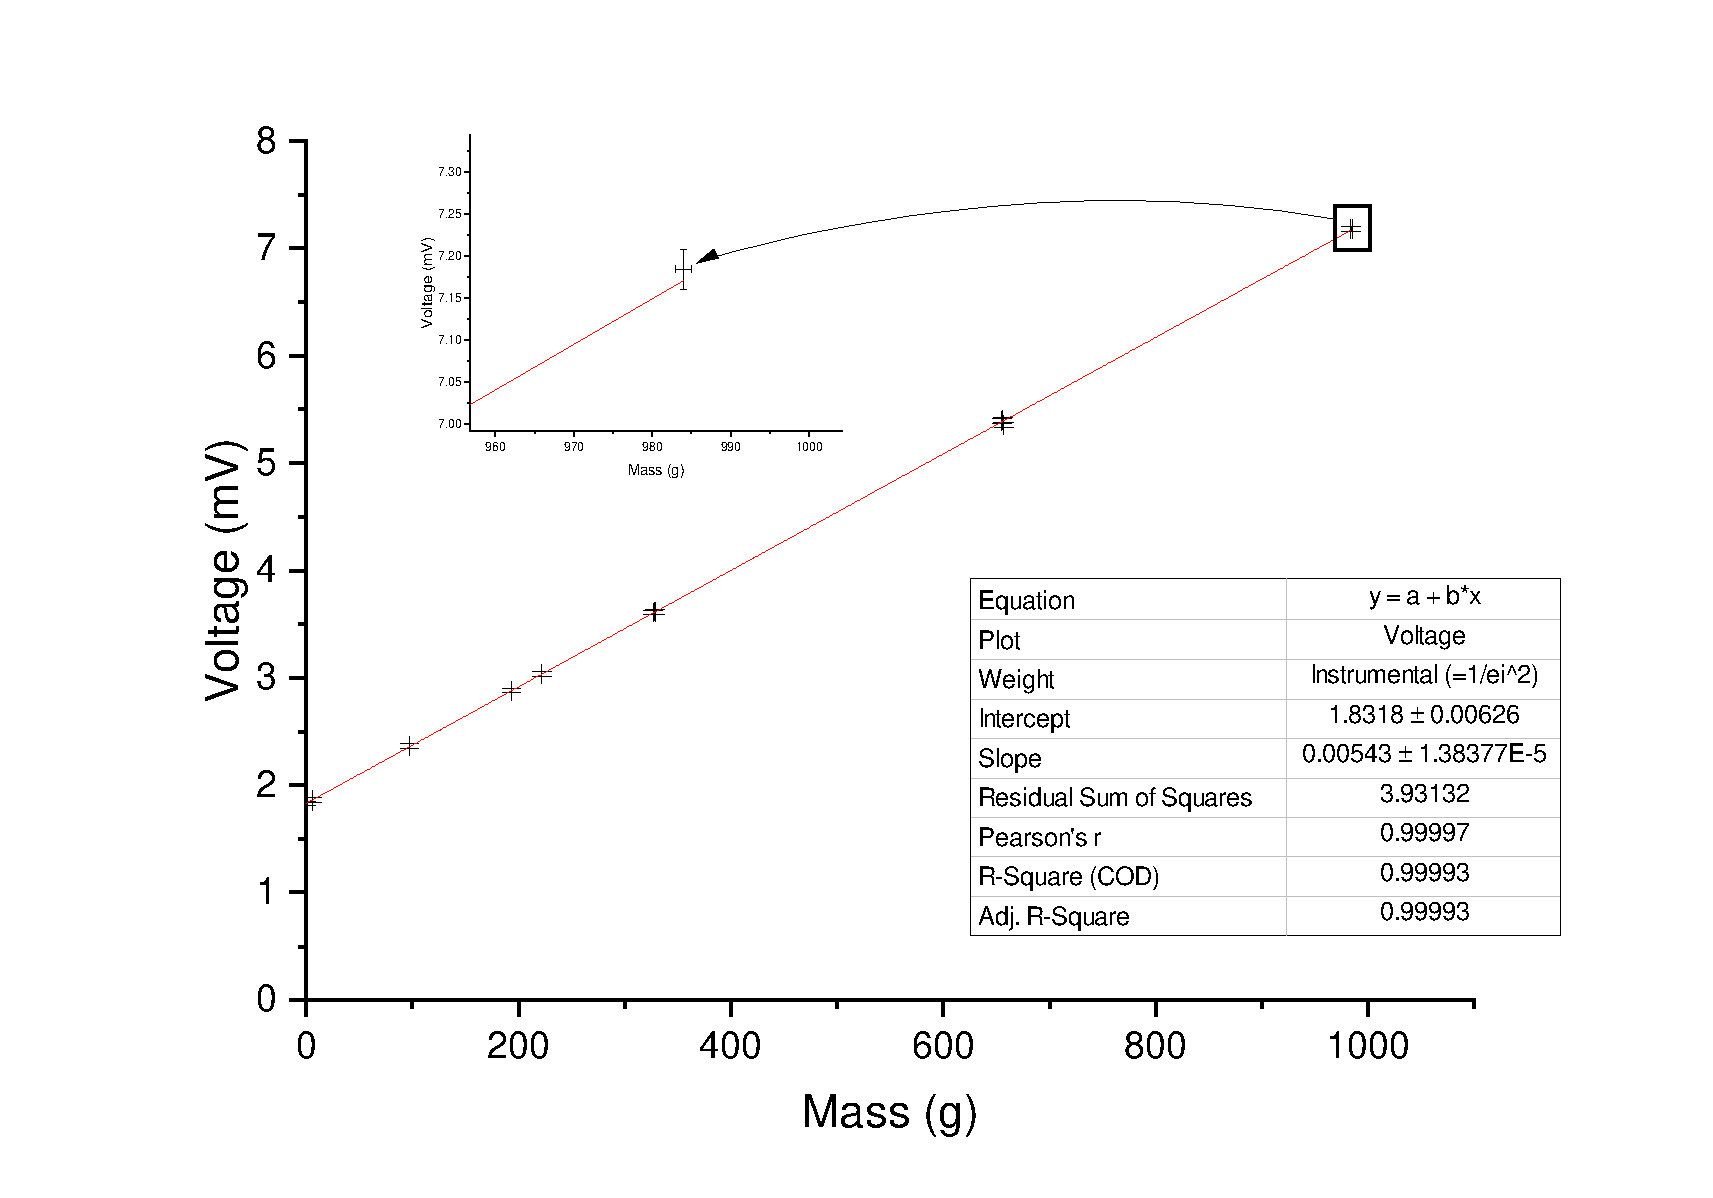
\includegraphics[width=\textwidth]{figures/beforeamp.pdf}
	\caption{Characteristic of our sensor before any amplification with the Wheatstone bridge exited at $E=3.33V$}
	\label{fig:beforeamp}
\end{figure}

%----------------------------------------------------------------%
\section{Amplifier}
\subsection{Theory of operation}
\paragraph{}
As seen in figure \ref{fig:beforeamp} the signal that outputs the Wheatstone bridge is a weak differential signal (mV).
\paragraph{}
We need to amplify it in order to get an acceptable signal for the Analog to Digital Converter.
The amplification is done by using a 3 AOP differential amplifier. The amplifier (MAX4194) is an SMD device which we used according to the schematics presented in \cite{MaximIntegrated-2015}.
\begin{figure}[H]
    \centering
    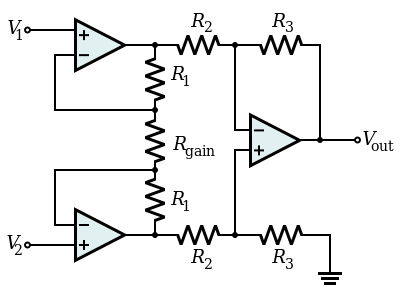
\includegraphics[width = .4\textwidth]{figures/3AOP_differential_amplifier.png}
    \caption{3 Amp op differential amplifier}
    \label{fig:3OpAmp}
\end{figure}
The difference of potential between the two branches is amplified according to this formula.
\begin{equation}
    \dfrac{V_{out}}{V_1-V_2}=(1+\dfrac{2R_1}{R_{gain}})\dfrac{R_3}{R_2}
\end{equation}
\subsection{Gain of the amplifier according to documentation}
In our case, we could only change the value of Rg as the differential amplifier is a component and not a circuit we had to make. The gain of this amplifier is calculated as follow:
\begin{equation}
    G=5+\dfrac{80000}{R_g}
\end{equation}
Knowing the maximum value that this amplifier can output as well as the maximum differential voltage of the Wheatstone bridge, it is possible to calculate the maximum gain authorized for our scale.
\begin{equation}
    Rg= \dfrac{80000}{G-5}
    \label{equ:rg}
\end{equation}
\begin{itemize}
    \item $R_g$ is the value of the gain resistance in $k\Omega$
    \item $G$ is the gain of the amplifier
    \item $80000$ is a value in $k\Omega$
\end{itemize}
The maximum mass we want to be able to measure is 1kg.
Using the linear regression extrapolated from the Wheatstone bridge (figure \ref{fig:Wheatstone}) we obtain that the differential voltage for 1kg is 7.26 mV.
As 3.33 V is the maximum output value of our differential, we obtain a maximum gain of 459.
Using (\ref{equ:rg}) we obtain a resistor of 176 $\Omega$. We do not have such resistor so we chose the closest higher resistor value we have at our disposal to not saturate the amplifier.
The value of Rg is 220 $\Omega$ which correspond to a gain of 369.
\begin{figure}[H]
    \centering
    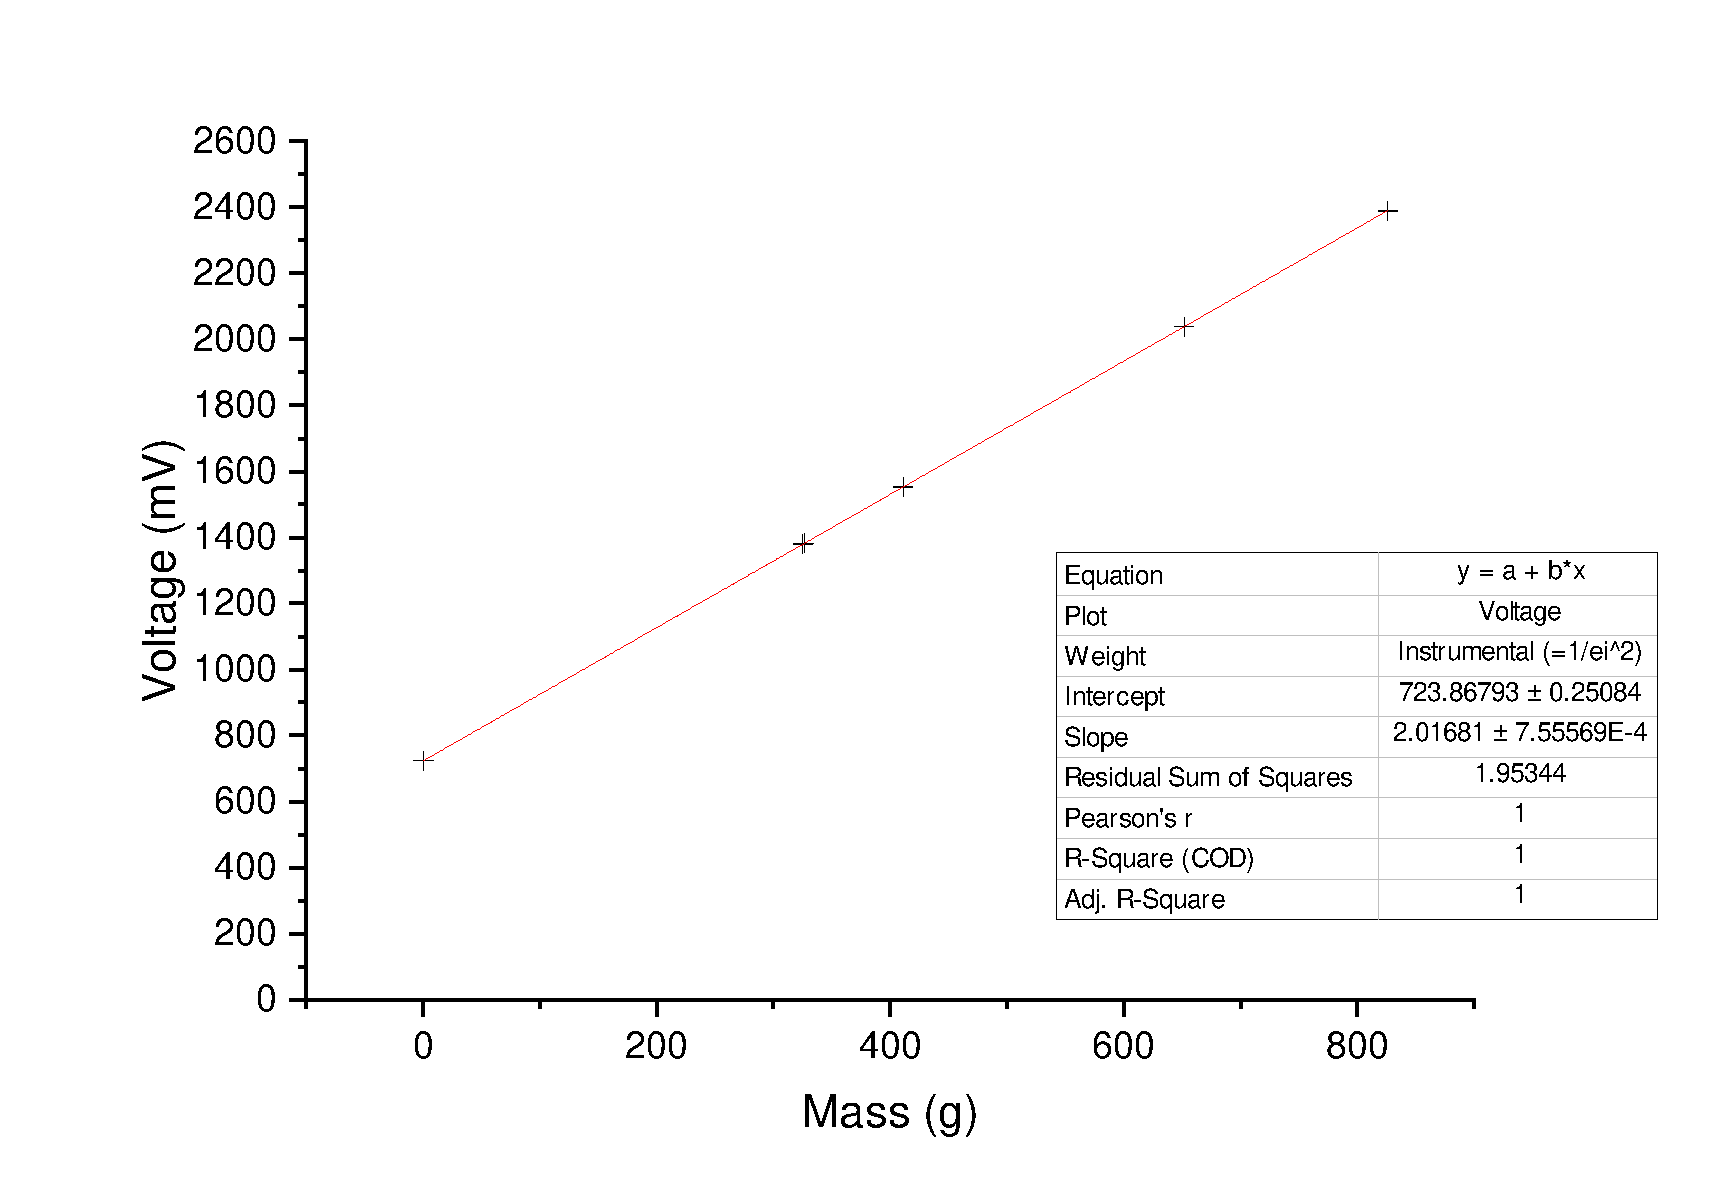
\includegraphics[width=.6\textwidth]{figures/offset_not_compensated.pdf}
    \caption{Amplified calibration of the scale}
    \label{fig:offset_not_compensated}
\end{figure}
We can see on figure \ref{fig:offset_not_compensated} that the signal is being correctly amplified, there is no saturation. However, we can observe an offset that can be caused by the strain of the platform on the strain gauge.
In order to correct this offset, we added a resistor in the Wheatstone bridge.
\begin{figure}[H]
    \centering
    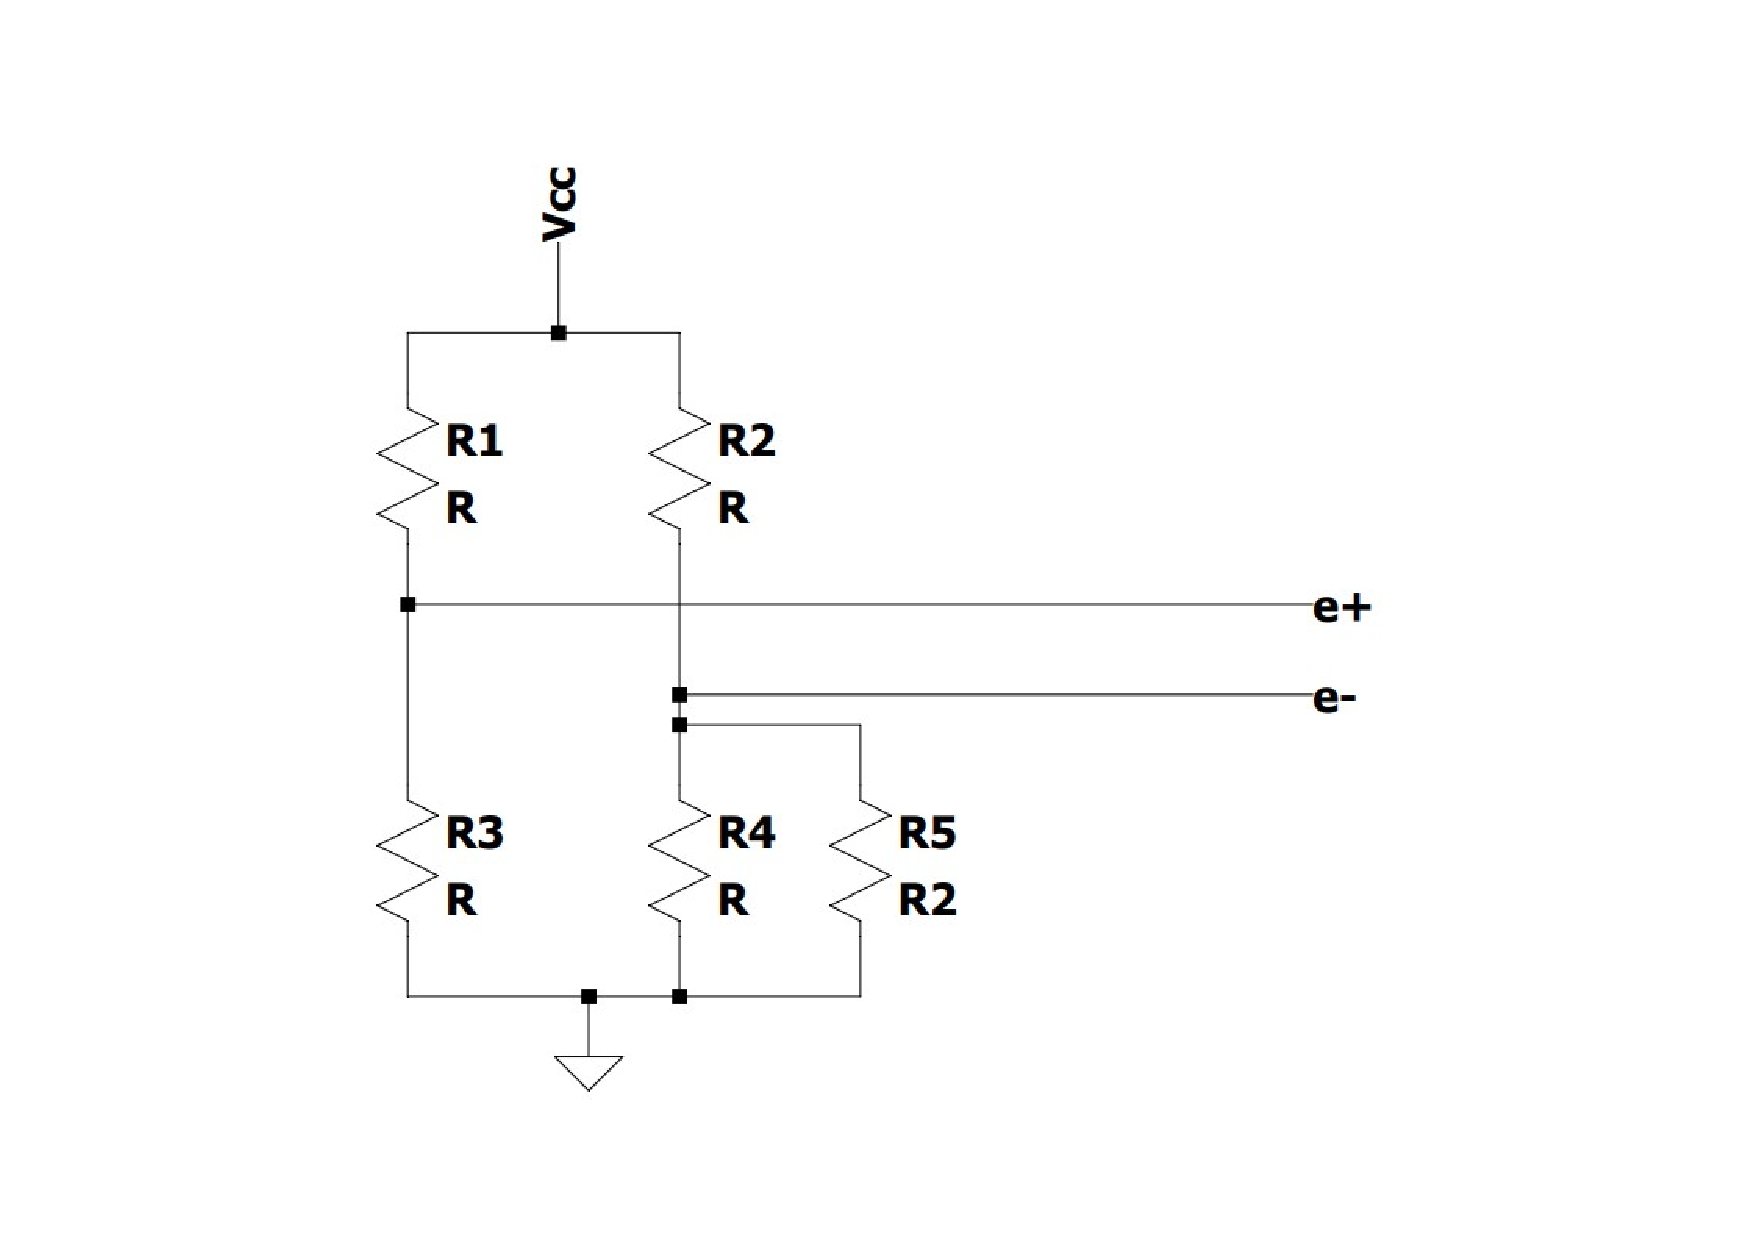
\includegraphics[width=.6\textwidth]{figures/Mod_Wheatstone.pdf}
    \caption{Modified Wheatstone bridge}
    \label{fig:Mod_Weatstone}
\end{figure}
This new resistor forms an equivalent resistor with R4 which helps us to readjust the potential in the node B to match the potential in node A so that the offset is negated.
We want to adjust around 0.002 mV so our resistor should be around 1M$\Omega$.
The value 470k$\Omega$ was empirically chosen.
We obtain the following result presented later in figure \ref{fig:final_calibration}.

%----------------------------------------------------------------%
\section{Analog to Digital Converter}
\subsection{Theory of operation}
\paragraph{}
Now that the signal is amplified, we can convert it into a digital signal via an Analog to Digital Converter (ADC).
The ADC is a $\Delta$$\Sigma$-ADC which means that the voltage value is converted into a linear amount of pulses during a period P. 
The higher the voltage the more pulses it outputs.
\paragraph{}
As seen in the schematic below, if we consider the signal to be constant, the integrator transforms it into a linear function.
Once that function reaches a threshold, a pulse is emitted, then each pulse is added to the output signal and by counting the amount of pulse (one pulse is equivalent to one quantum of voltage) it is possible to find the voltage.\\
\paragraph{}
The shape of the digitized signal is described by a step function. Due to the shape, an error is induced by the difference between the value and the closest digital value of the conversion device. The noise is called quantification noise and is equal to 1 quantum in the worst case scenario.
\begin{figure}[H]
    \centering
    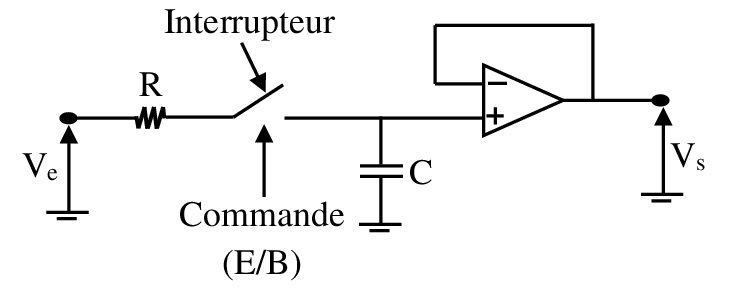
\includegraphics[width=.6\textwidth]{figures/echantilloneur.png}
    \caption{Sampling device schematic \cite{book}}
    \label{fig:CAN_ech}
\end{figure}

We can have $2^{16}$ values from 0 to 2.048 V so our quantum is 31.2 $\mu$V.
\begin{figure}[H]
    \centering
    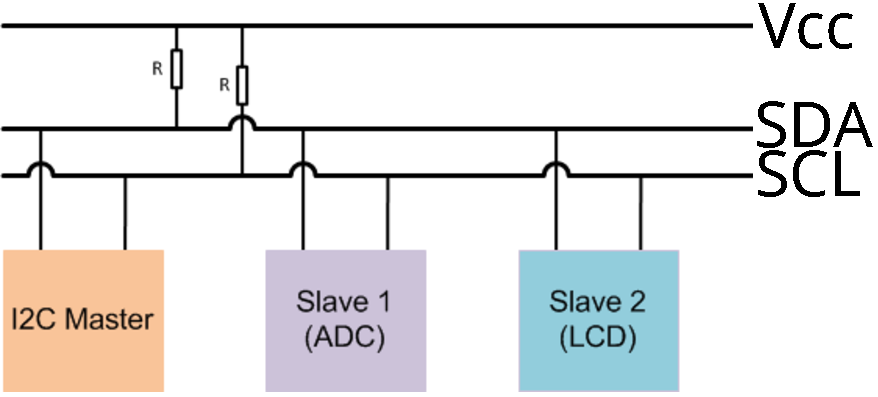
\includegraphics[width=.5\textwidth]{figures/i2c_diagram.pdf}
    \caption{$I^2C$ schematic courtesy of \cite{Matworks-2022}}
    \label{fig:i2c_diagram}
\end{figure}
The ADC uses the $I^2C$ protocol to convey information to the mother board. 
The $I^2C$ protocol revolves around two wires that connects one master (the mother board here) and slaves (the ADC). 
One transfer data while the clock signal is in the other.
Each slave has an address that the master uses to call it whenever it needs it.
Each bit of data bus is given by a voltage, if there is 0V it is considered to be 0 and if there is a voltage it is a 1.
The signal created is now a logical signal that can be translated by the master.
The signal is composed of a start bit then the address of the slave in binary then the slave respond via a bit called ACK.
The clock signal is used to read the data sent.
It is then possible to have more than one slave with only two wires (We will not use this feature here).
In order to have these two different voltages, we use two resistor connected to Vcc and the wires.
Each wire can be connected to the ground so that the voltage can be 0V (bit 0) or not 0V (bit 1), the pull up resistor prevent short-circuiting and fix the bit to 1 when no one send data through the wires.
\begin{figure}[H]
    \centering
    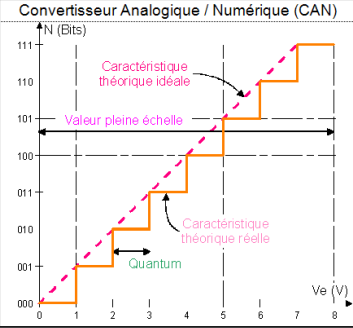
\includegraphics[width=.4\textwidth]{figures/CAN.png}
    \caption{Analogue to digital conversion modelized by a step function \cite{CedricKillian-2020}}
    \label{fig:CAN_step}
\end{figure}
%----------------------------------------------------------------%
\section{Noise reduction}
\paragraph{}
A lab is isolated from a lot of external noise. In order to reinforce the noise reduction capability of our weighting scale, we must add some noise sources to see and reduce the effects. We will be focusing on two noise sources : a vibration generator and an electromagnetic noise generator.
\subsection{Mechanical vibrations}
\paragraph{}
A small electric motor with a mass is added near the sensor. A non-symmetrical mass is placed on the rotor in order to create a distance between the centre of rotation and the gravity centre of the mass. When rotating, this device produces vibrations. Using the stroboscopic effect of our smartphone camera (at 60 frames per second) we set the motor speed at 60Hz.
\paragraph{}
The periodic nature of the synthetic noise is easily quantified using Fast Fourrier Transform algorithm on a long enough signal sample (1s in our case).
The results are the following :
\begin{figure}[H]
\centering
\begin{subfigure}{.5\textwidth}
  \centering
  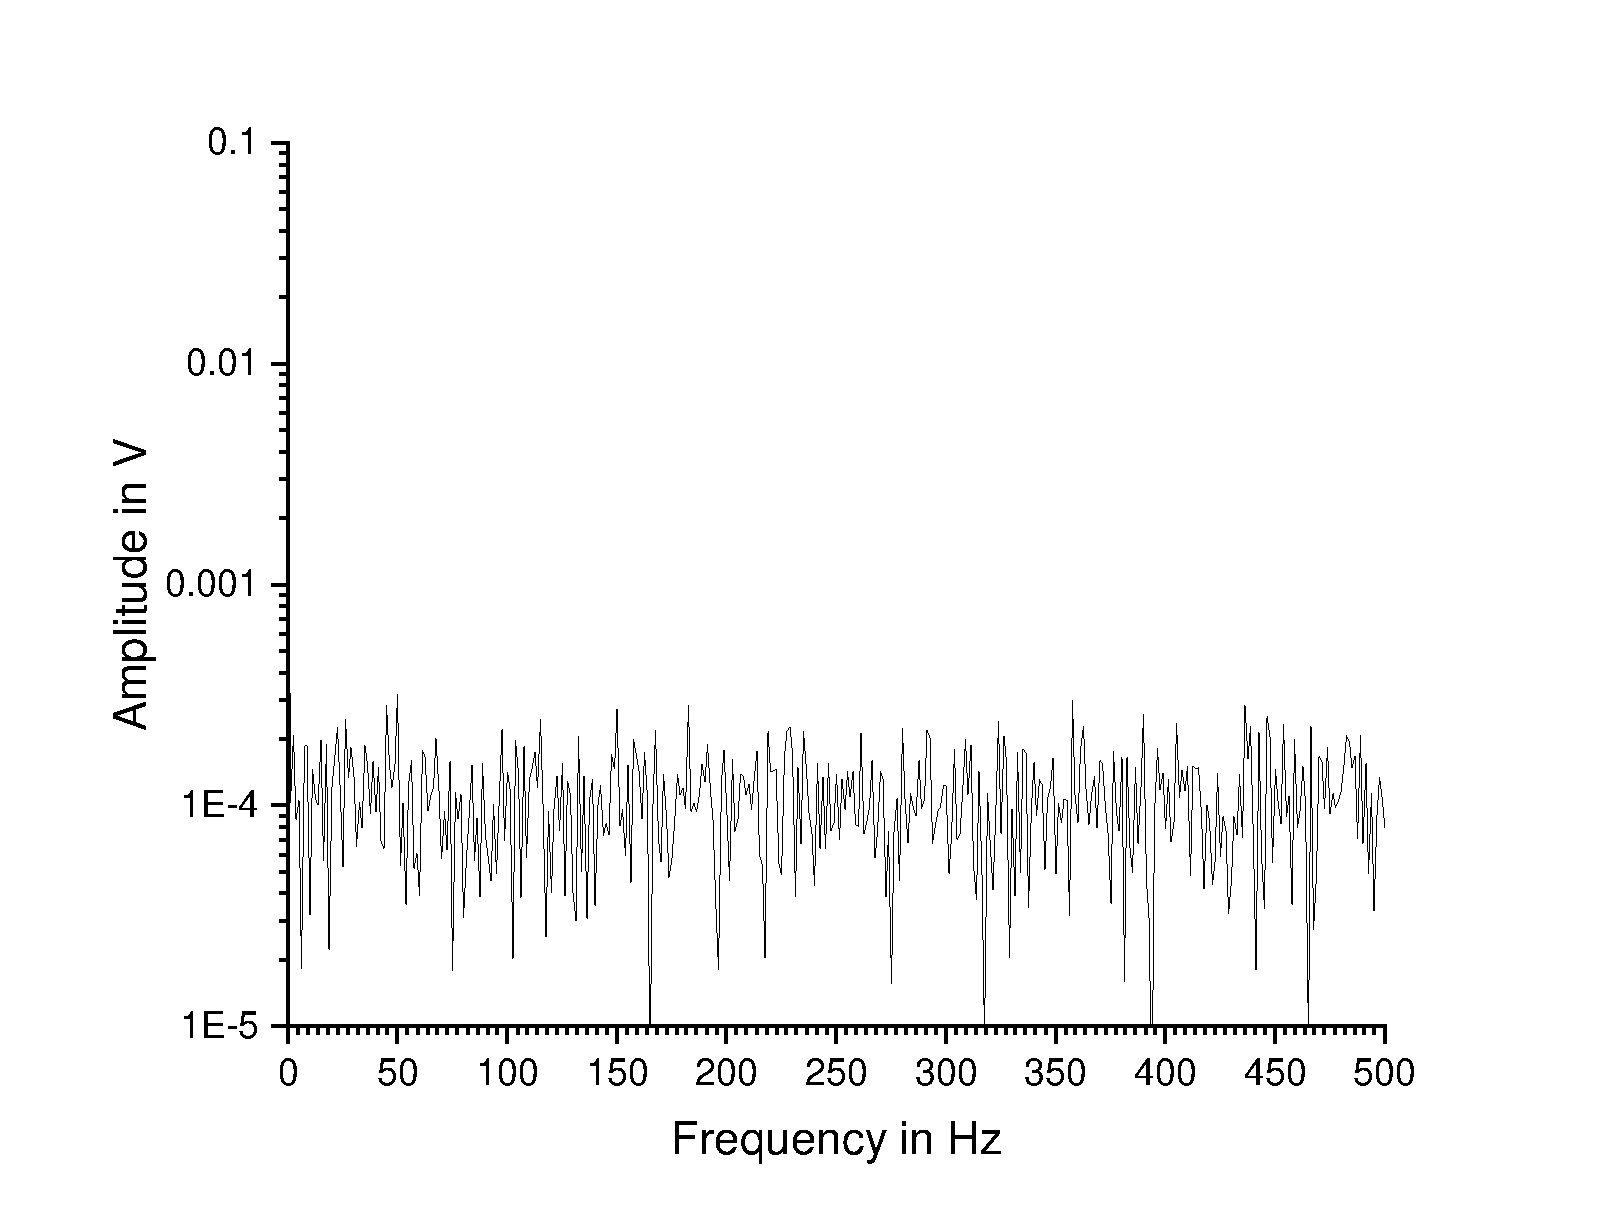
\includegraphics[width=\linewidth]{figures/nomotornofilter.pdf}
  \caption{FFT of the recovered signal before digitalization\\ without the motor}
  \label{fig:nomotornofilter}
\end{subfigure}%
\begin{subfigure}{.5\textwidth}
  \centering
  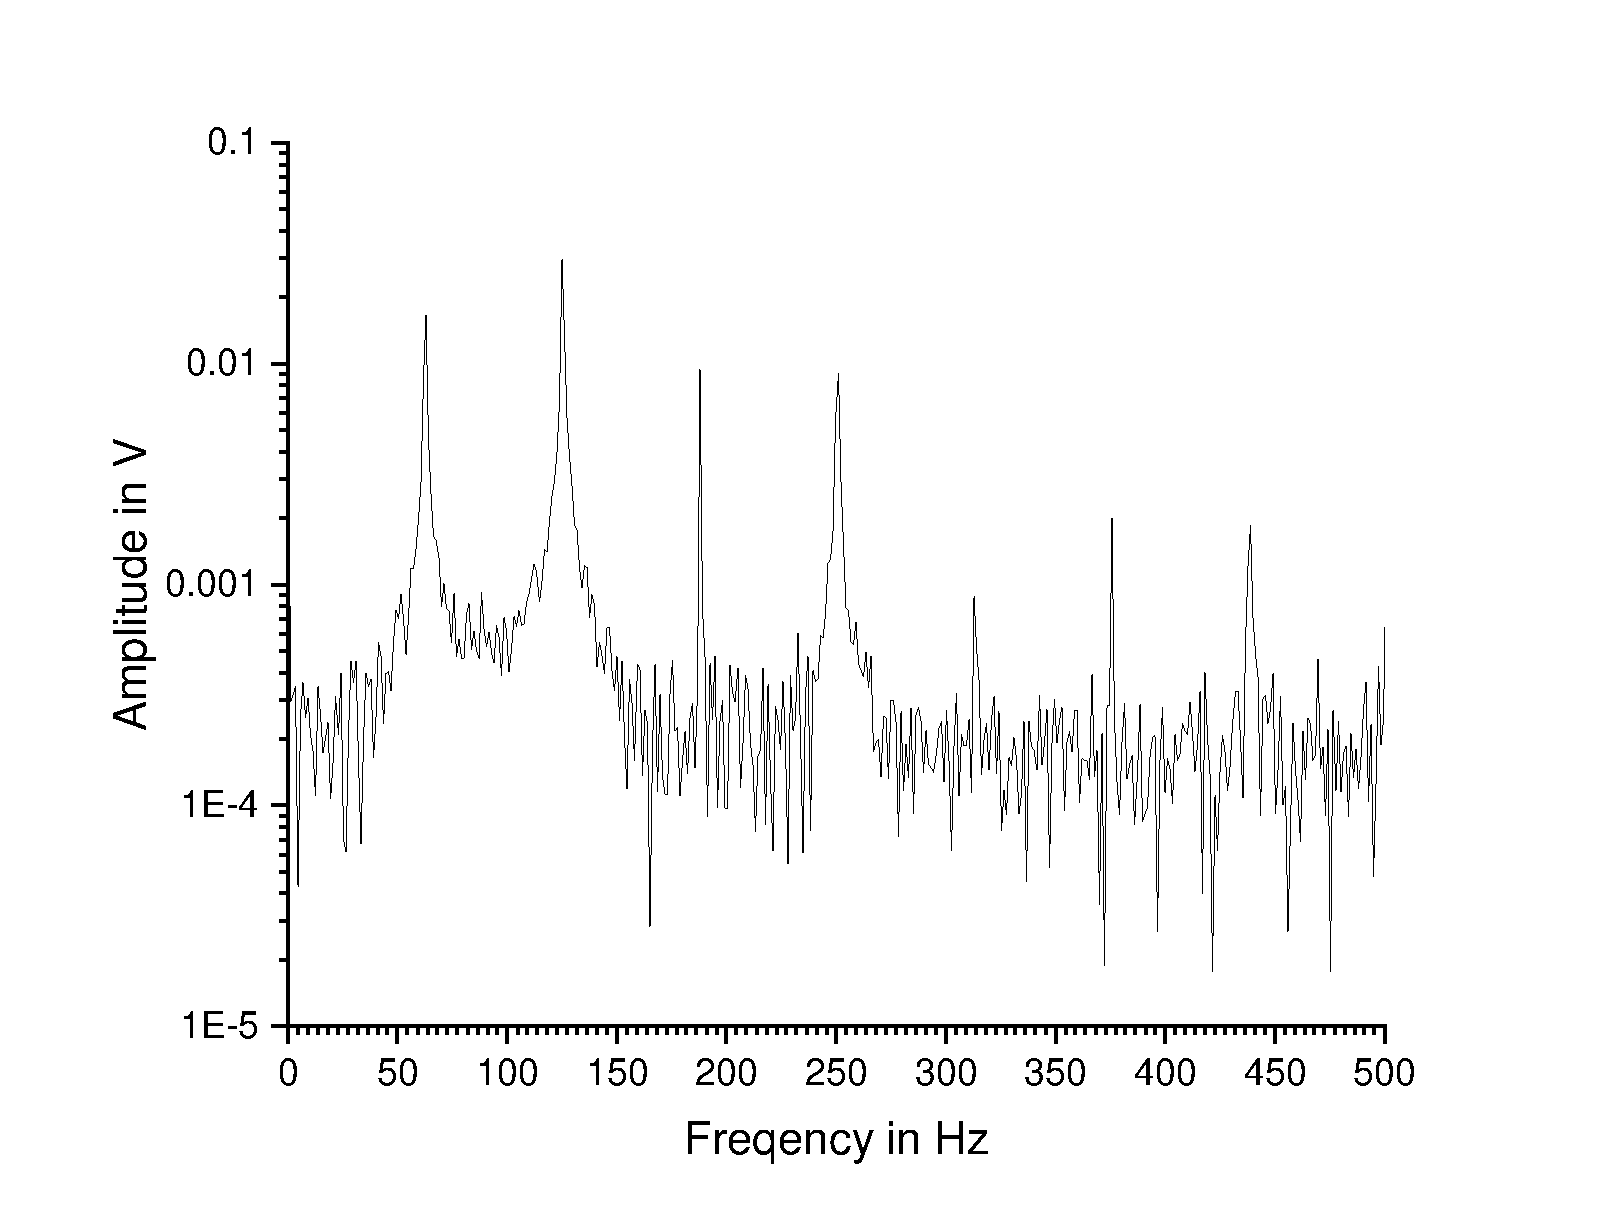
\includegraphics[width=\linewidth]{figures/motornofilter.pdf}
  \caption{FFT of the recovered signal before digitalisation\\ with the motor at 60 rounds per second}
  \label{fig:motornofilter}
\end{subfigure}
\caption{}
\label{fig:nofilterFFT}
\end{figure}
Figure \ref{fig:nofilterFFT} shows an evident spectral contribution of the vibration device we added. In addition, we observed the standard deviation of a weigh measurement. We acquired more than 30 values in each cases for determination of an experimental standard variation using the SD formula of our data processing software : $s = \sqrt{\frac{1}{n-1} \sum_{i=1}^n (x_i - \overline{x})^2}$. \\
\begin{center}
\begin{tabular}{|c|c|}
    \hline
    Without motor & With Motor \\
    \hline
     $1.20$mV & $3.39$mV \\
    \hline
\end{tabular}
\end{center}
\paragraph{}
Since the useful part of the signal is only in the DC component. A Low-Pass filter should eliminate the disturbance while keeping the information in the signal.
\paragraph{}
In accordance with the available components, an RC filter ($1^{st}$ order) with a cutoff frequency of $0.8Hz$ is added to the circuit. Same measurements are made with after the filter is soldered on the board. Results are the following : 
\begin{figure}[H]
\centering
\begin{subfigure}{.5\textwidth}
  \centering
  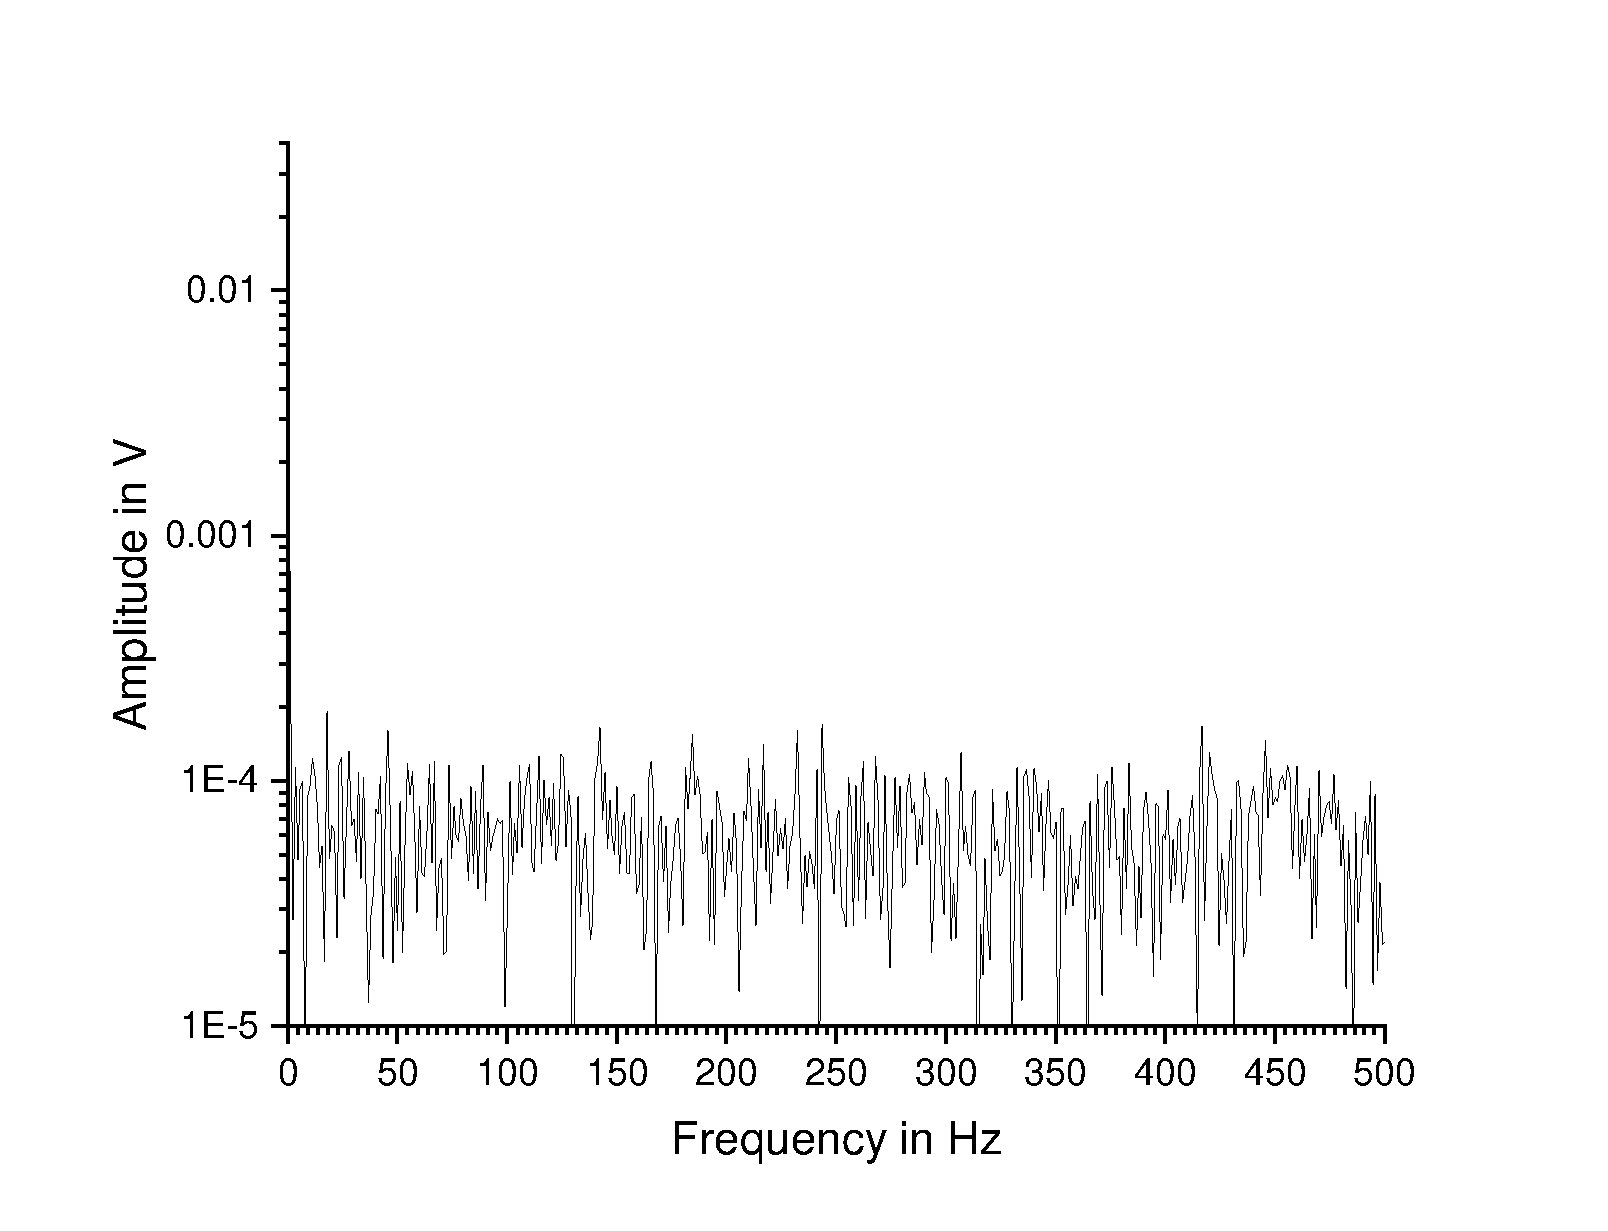
\includegraphics[width=\linewidth]{figures/nomotorfilter.pdf}
  \caption{FFT of the recovered signal before digitalization\\ without the motor}
  \label{fig:nomotornofilter2}
\end{subfigure}%
\begin{subfigure}{.5\textwidth}
  \centering
  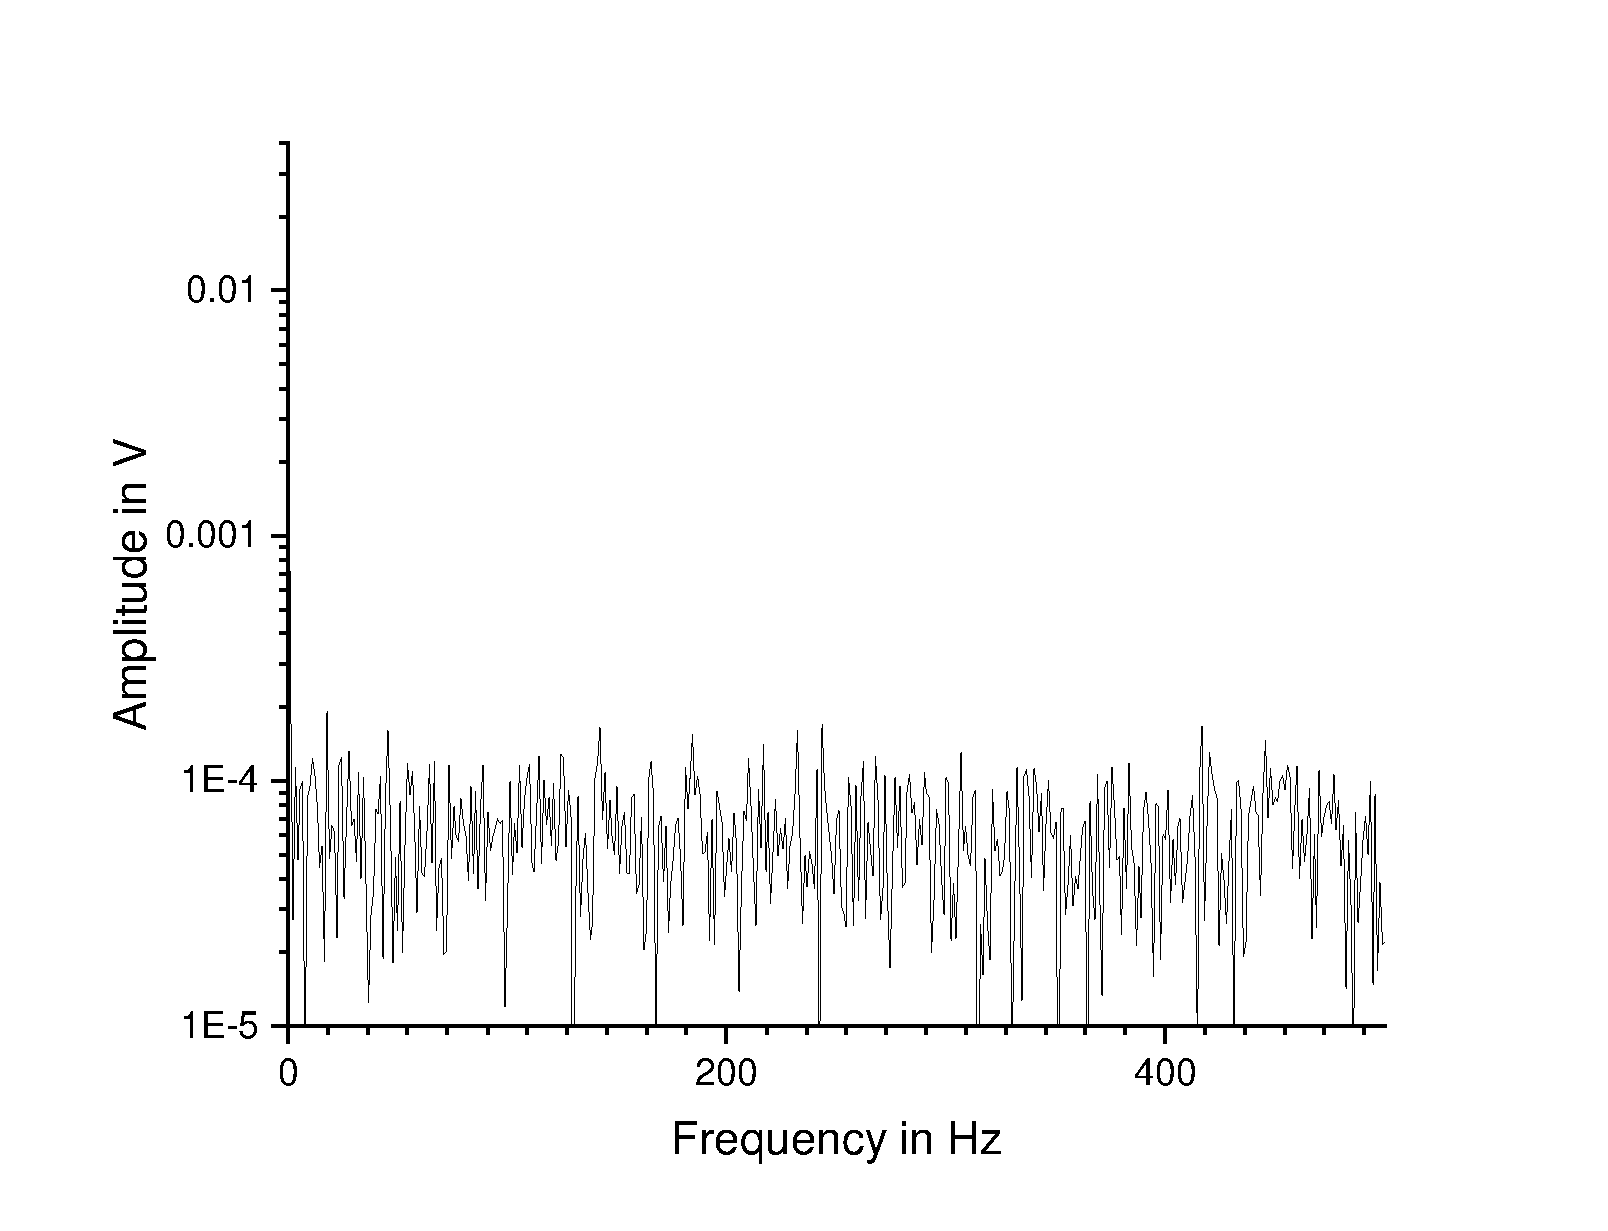
\includegraphics[width=\linewidth]{figures/motorfilter.pdf}
  \caption{FFT of the recovered signal before digitalisation\\ with the motor at 60 rounds per second}
  \label{fig:motornofilter2}
\end{subfigure}
\caption{With the RC Low-Pass filter}
\label{fig:filterFFT}
\end{figure}
Figure \ref{fig:filterFFT} shows the absence of AC component noise in our signal. Howerver, with the filter the stabilisation of the value takes more time. We must wait $3\tau$ to get a stable value. On the other hand, the displayed value seemed more stable. The same standard deviation measurement was made and the results showed a reduced variance of both values.
\begin{center}
\begin{tabular}{|c|c|}
    \hline
    Without motor & With Motor \\
    \hline
     $0.095$mV & $0.109$mV \\
    \hline
\end{tabular}
\end{center}
The Motor contribution to the variance of the measurement system is completely wiped thanks to the low pass filter.
\subsection{Electromagnetic noise}
Electric motors are made with carbon brushes to make an electrical contact between the static wires and the moving parts. Because the contact is not always perfect, some sparks may occur randomly in the enclosure of the motor. Sparks can be assimilated as electromagnetic Diracs of high intensity. Using a large enough time-span, we can observe the sparks being transmitted by electromagnetic waves to the copper of the printed circuit board. The time span must not be too wide because the probability of the oscilloscope skipping a spark between two points increases with the sampling frequency. Figure \ref{fig:sparks} show some sparks acquired on the oscilloscope.
\begin{figure}[H]
    \centering
    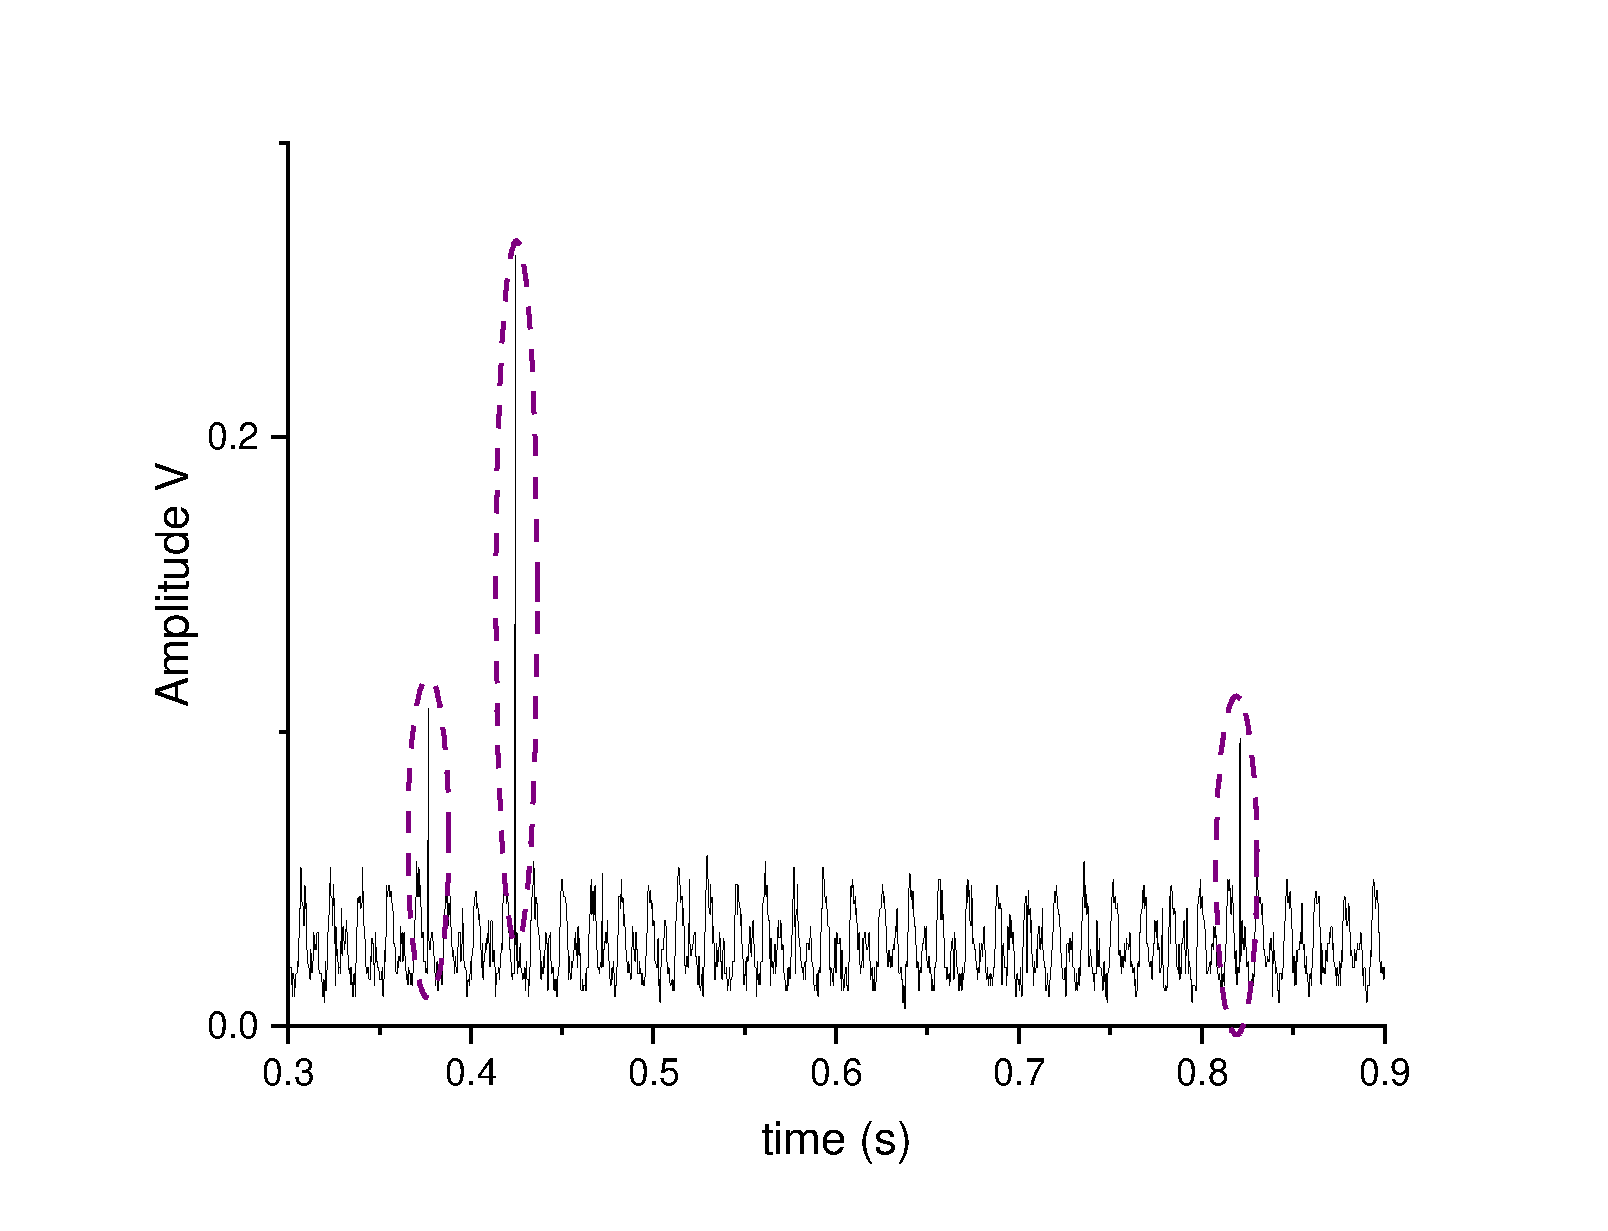
\includegraphics[width=0.6\textwidth]{figures/sparks.pdf}
    \caption{in Violet dashes : EM Sparks triggered by the brushes of the electric motor}
    \label{fig:sparks}
\end{figure}
\paragraph{}
To reduce the sparks effect, a proof-of-concept faraday cage was made using steel plates. 
\begin{figure}[H]
\centering
\begin{subfigure}{.5\textwidth}
  \centering
  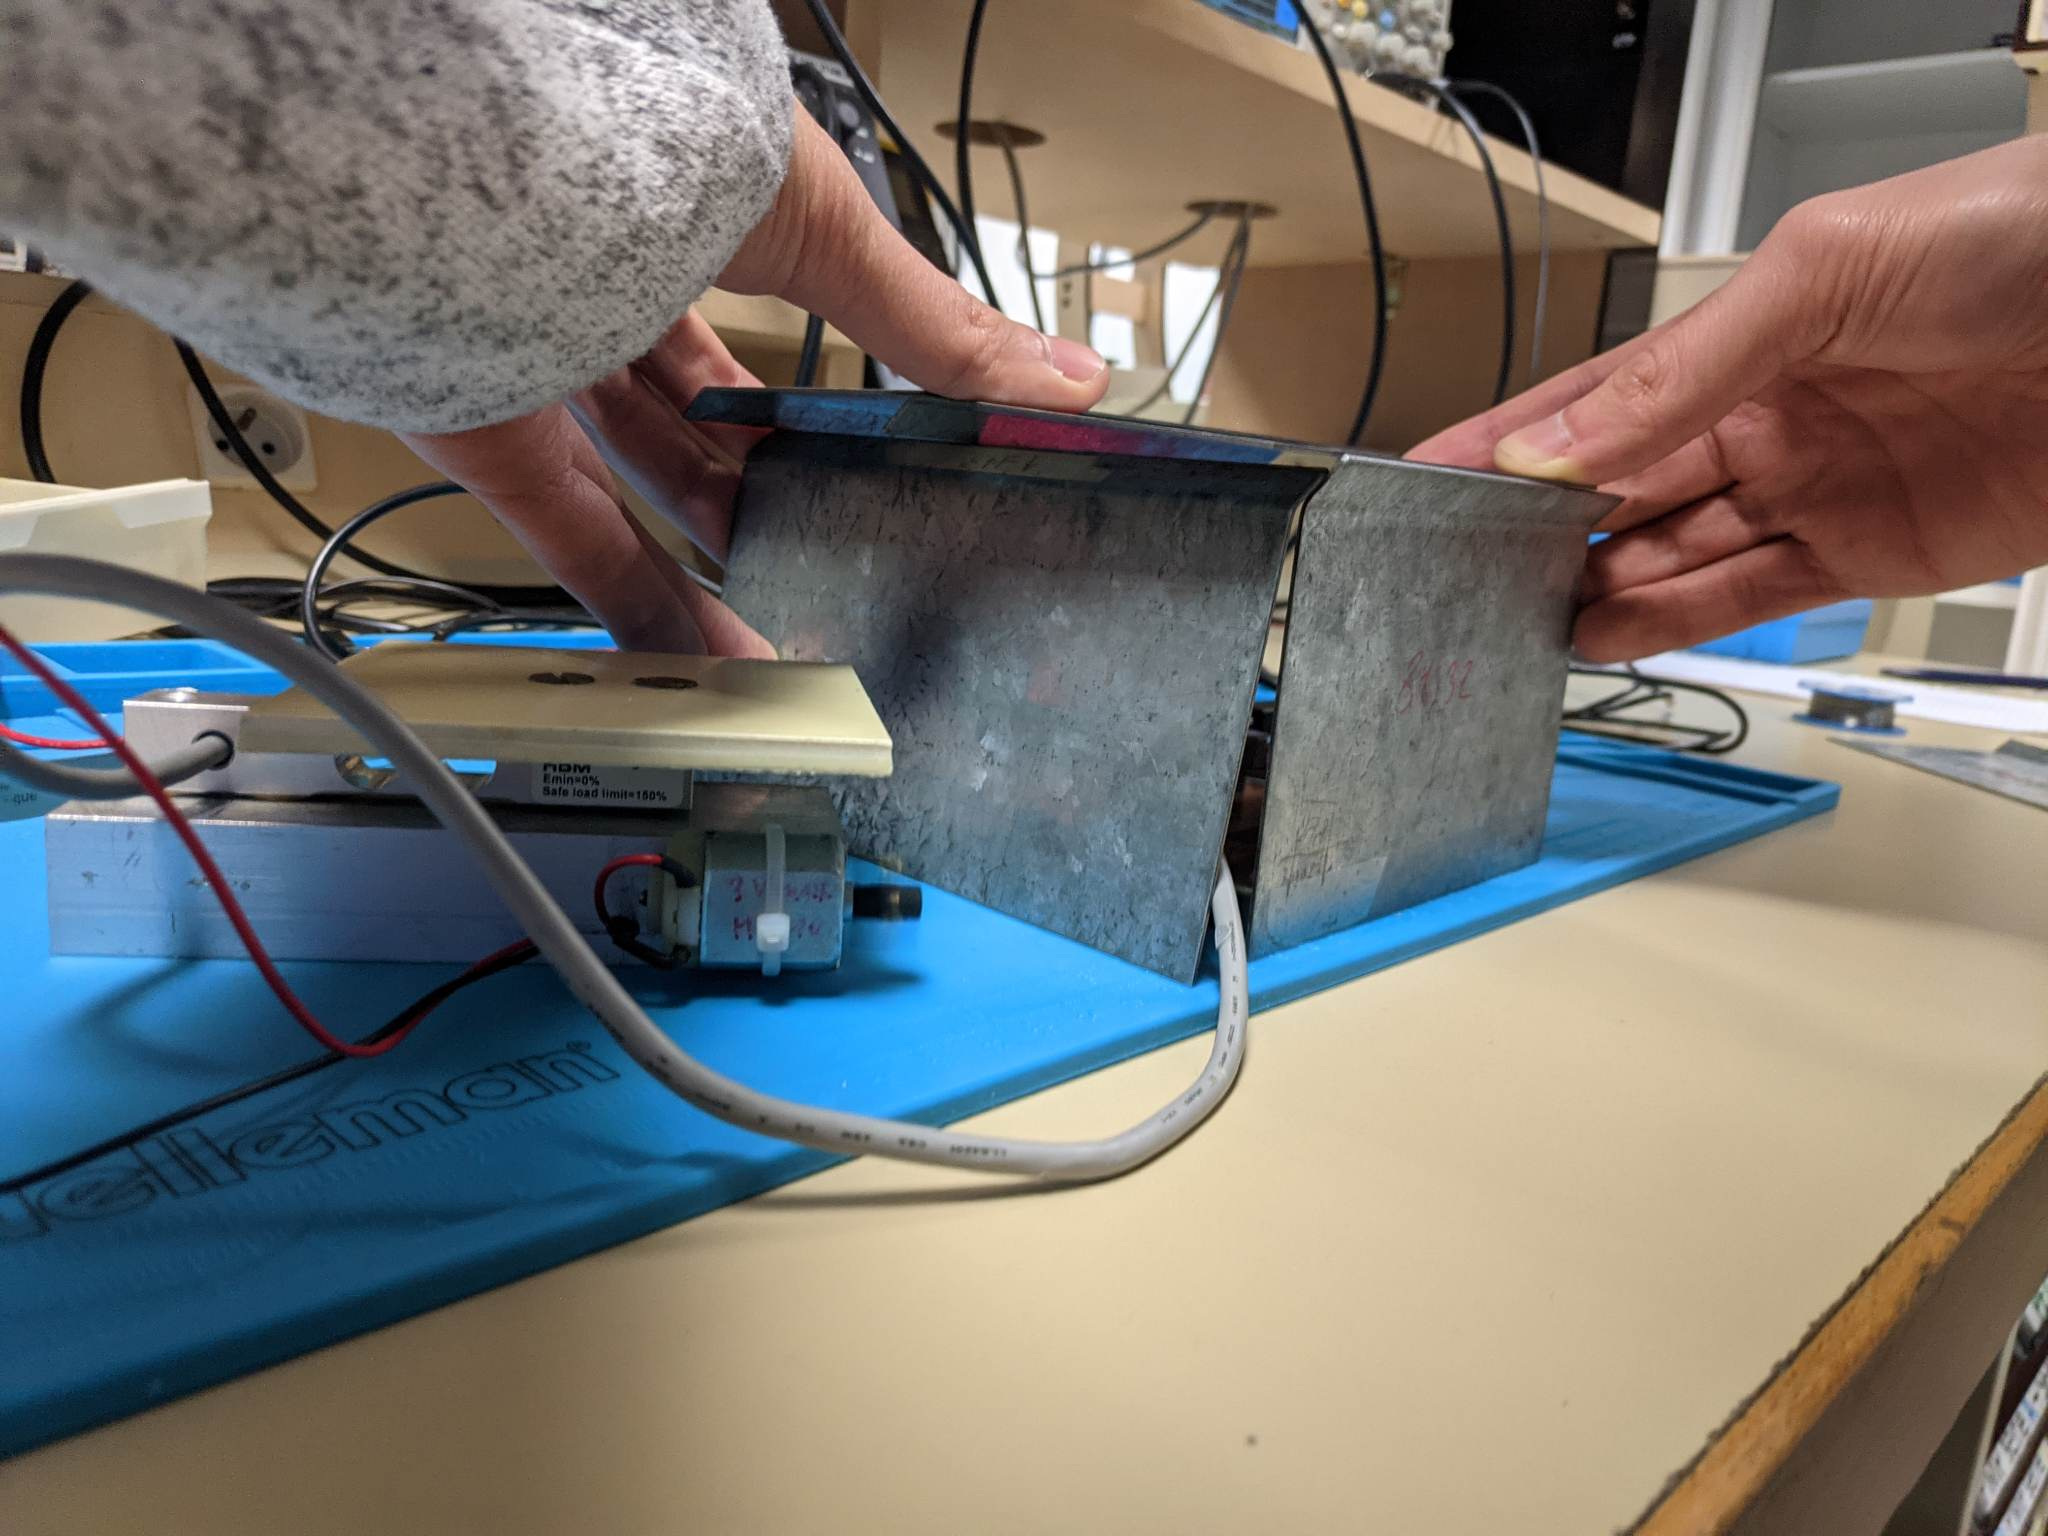
\includegraphics[width=\linewidth]{figures/faraday.jpg}
  \caption{Picture of the faraday cage setup arround the printed circuit board}
  \label{fig:faradaypic}
\end{subfigure}%
\begin{subfigure}{.5\textwidth}
  \centering
  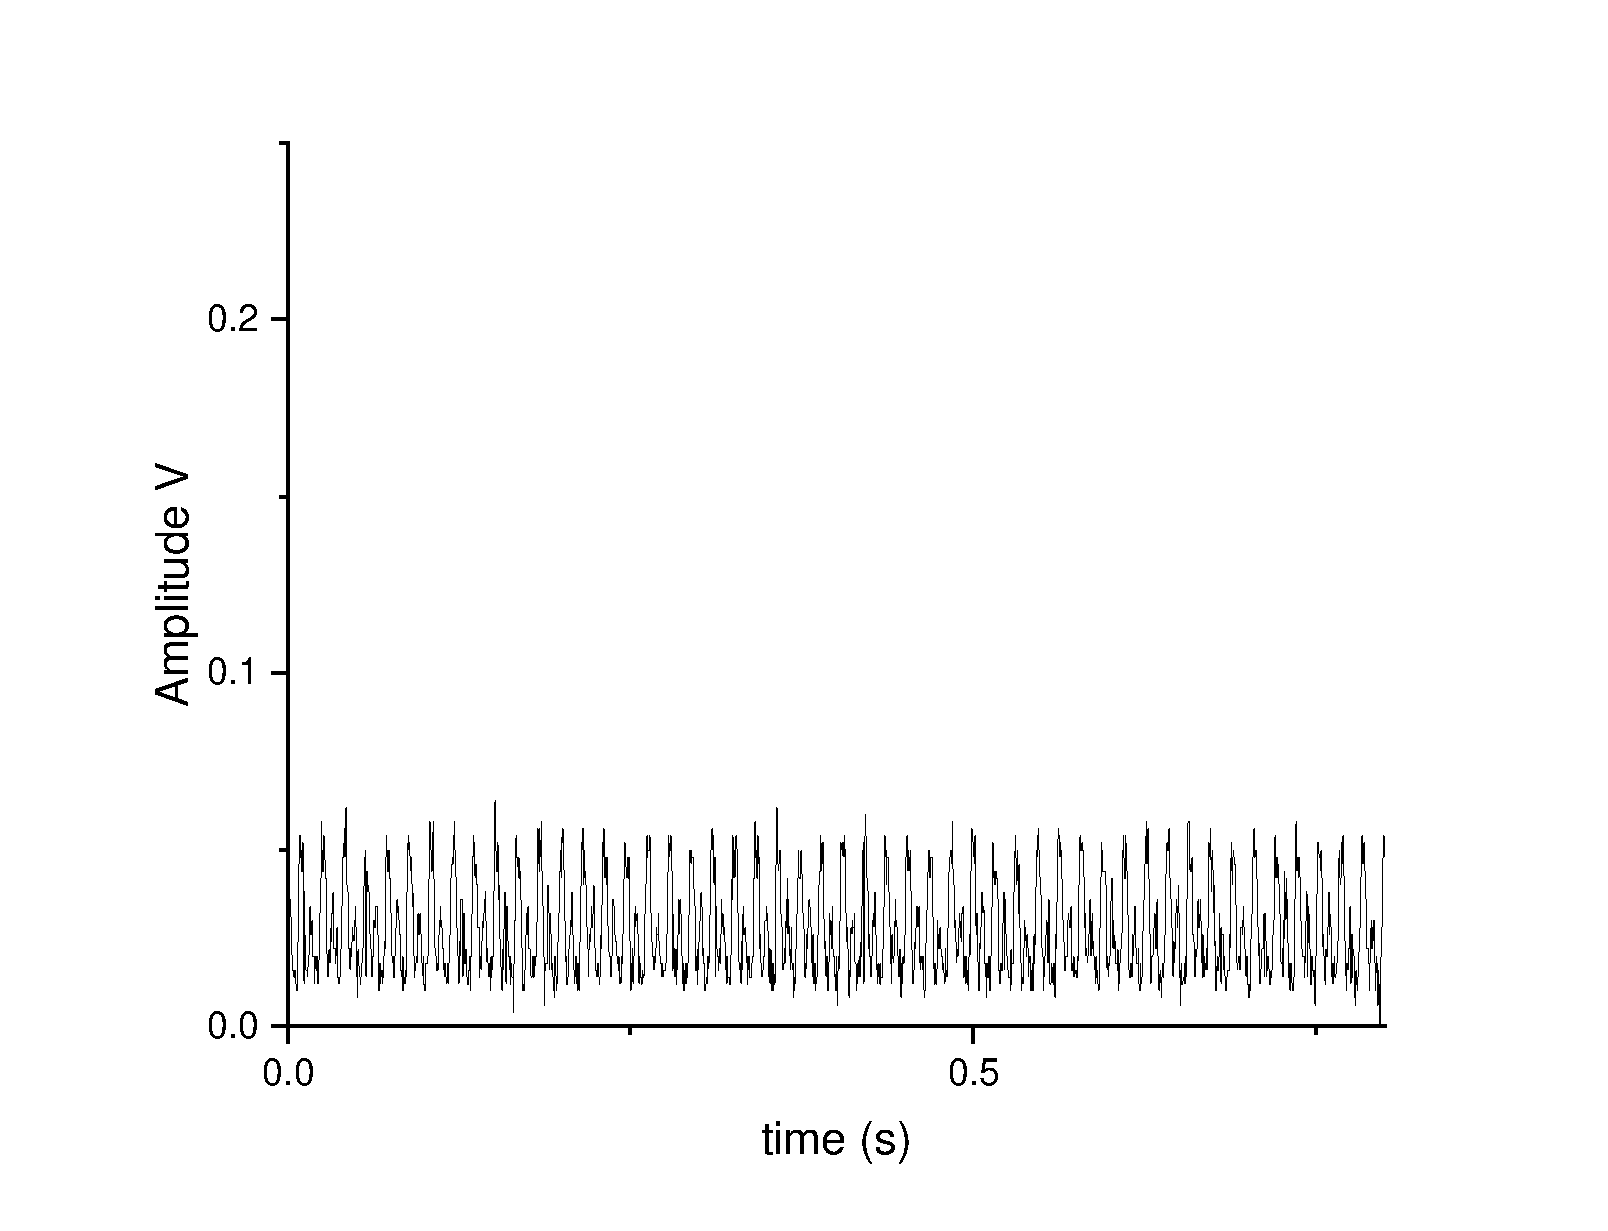
\includegraphics[width=\linewidth]{figures/faraday.pdf}
  \caption{Signal with absence of sparks}
  \label{fig:faradaysig}
\end{subfigure}
\caption{}
\label{fig:faraday}
\end{figure}
\paragraph{}
The data proves that a metallic shield provide good insulation against such EM disturbances. We could consider integrating it in the final product.
%----------------------------------------------------------------%
\section{Error Budget}
\paragraph{}
The prototype is now fully completed. The layout of the PCB is drawn on figure \ref{fig:layout}
\begin{figure}[H]
    \centering
    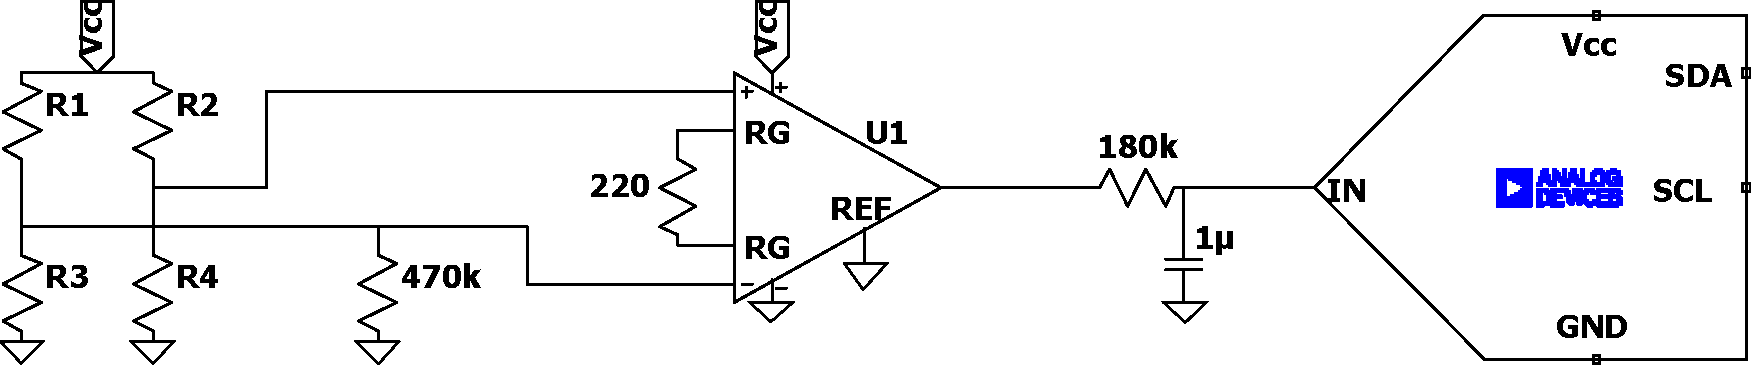
\includegraphics[width=\textwidth]{figures/layout.pdf}
    \caption{Layout of our printed circuit board}
    \label{fig:layout}
\end{figure}
The thermal noise or Johnson–Nyquist noise affects only resistive components \cite{Bucci-2020}. The RMS Voltage resulting of the noise is given by :
\begin{equation}
    V_{noise}=\sqrt{4Rk_bT\Delta f}
\end{equation}
\begin{itemize}
    \item $\Delta f$ Bandwidth in Hertz
    \item $R$ Resistance in Ohm
    \item $k_b$ Boltzmann's Constant : $1.380649.10^{-23} J.K^{-1}$ 
    \item $T$ Temperature in Kelvin
\end{itemize}

%INSERT BuDGET ERROR HERE
The differential amplifier can be modelled this way to take into account the different imperfections of the amplifier.
The values can be found in the amplifier's datasheet.
\begin{figure}[H]
    \centering
    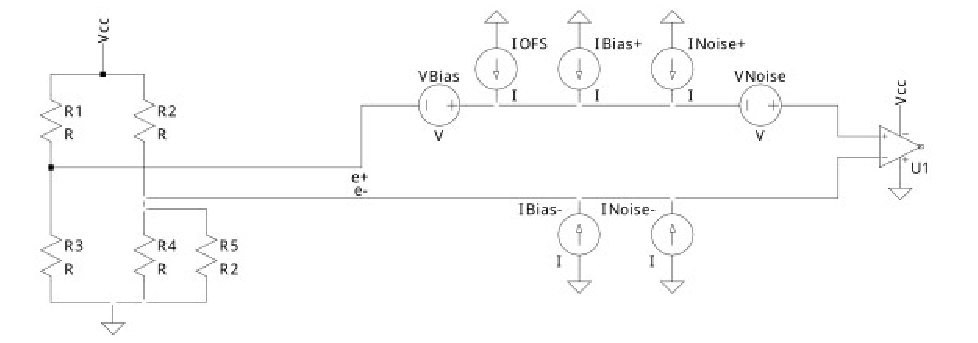
\includegraphics[width=0.9\textwidth]{figures/error_budget.pdf}
    \label{fig:error_budget}
    % pour info J'ai crop ta figure il y avait des marges trop grosses
    \caption{amplifier error schematic}
\end{figure}
\begin{itemize}
    \item $V_{INoise+}$ = 0.21 nV
    \item $V_{INoise-}$ = 0.21 nV
    \item $V_{Bias+}$ = 14 $\mu$V
    \item $V_{Bias-}$ = 14 $\mu$V
    \item $V_{Noise}$ = 0.35 $\mu$V
    \item $V_{OFS}$ = 164 $\mu$V
    \item $V_{IOFS}$ = 1.25 $\mu$V
\end{itemize}
Each component of the error can be calculated separately, then the squared values can be summed up to obtain the total error budget of the system.
\begin{equation}
    Er_{tot}=\sqrt{V_{INoise+}^2 + V_{INoise-}^2 + V_{Bias+}^2 + V_{Bias-}^2 + V_{Noise}^2 + V_{OFS}^2 + V_{IOFS}^2}
\end{equation}
The total error budget sum up to 1.65 $\mu$V for a maximum signal amplitude of 7.26 mV.
\begin{equation}
    Er_{bud}=100*\dfrac{Er_{tot}}{V_{maxsig}}
\end{equation}
\begin{itemize}
    \item $Er_{bud}$ is the error budget in percentage
    \item $Er_{tot}$ is the total error in mV
    \item $V_{maxsig}$ is the maximum value of the useful signal
\end{itemize}
We obtain this value:
\begin{equation}
    Er_{bud}=2.27\%
\end{equation}
The thermal noise generated by the resistors is negligible with respect to the amplifier noise.

We can describe the error in terms of affected quantum. In our case, the 16 bit resolution of the conversion devices allows us to neglect the quantification error with respect to the electrical noise. We can therefore calculate the amount of noise in quantum units, and we will determine the Signal to noise ratio between the number of affected quantum and $2^{16}$ bits. In our case, the error is affecting 19 digits. We can round up to 20 digits because of the quantification error that is in the worst case 1 quantum. I term of mass, we can say that this device is able to detect a variation of 0.32 grams.
%----------------------------------------------------------------%
\section{Conclusion}
\subsection{Final calibration of the weighting scale}
\paragraph{}
Finally, we can produce a calibration curve for our device. Strain gauges are very sensitive sensors that provide a very good linearity on a wide mesurand span. We obtained a $R^2=1$ which means that all the variation in the y values is accounted for by the x values. 
\begin{figure}[H]
    \centering
    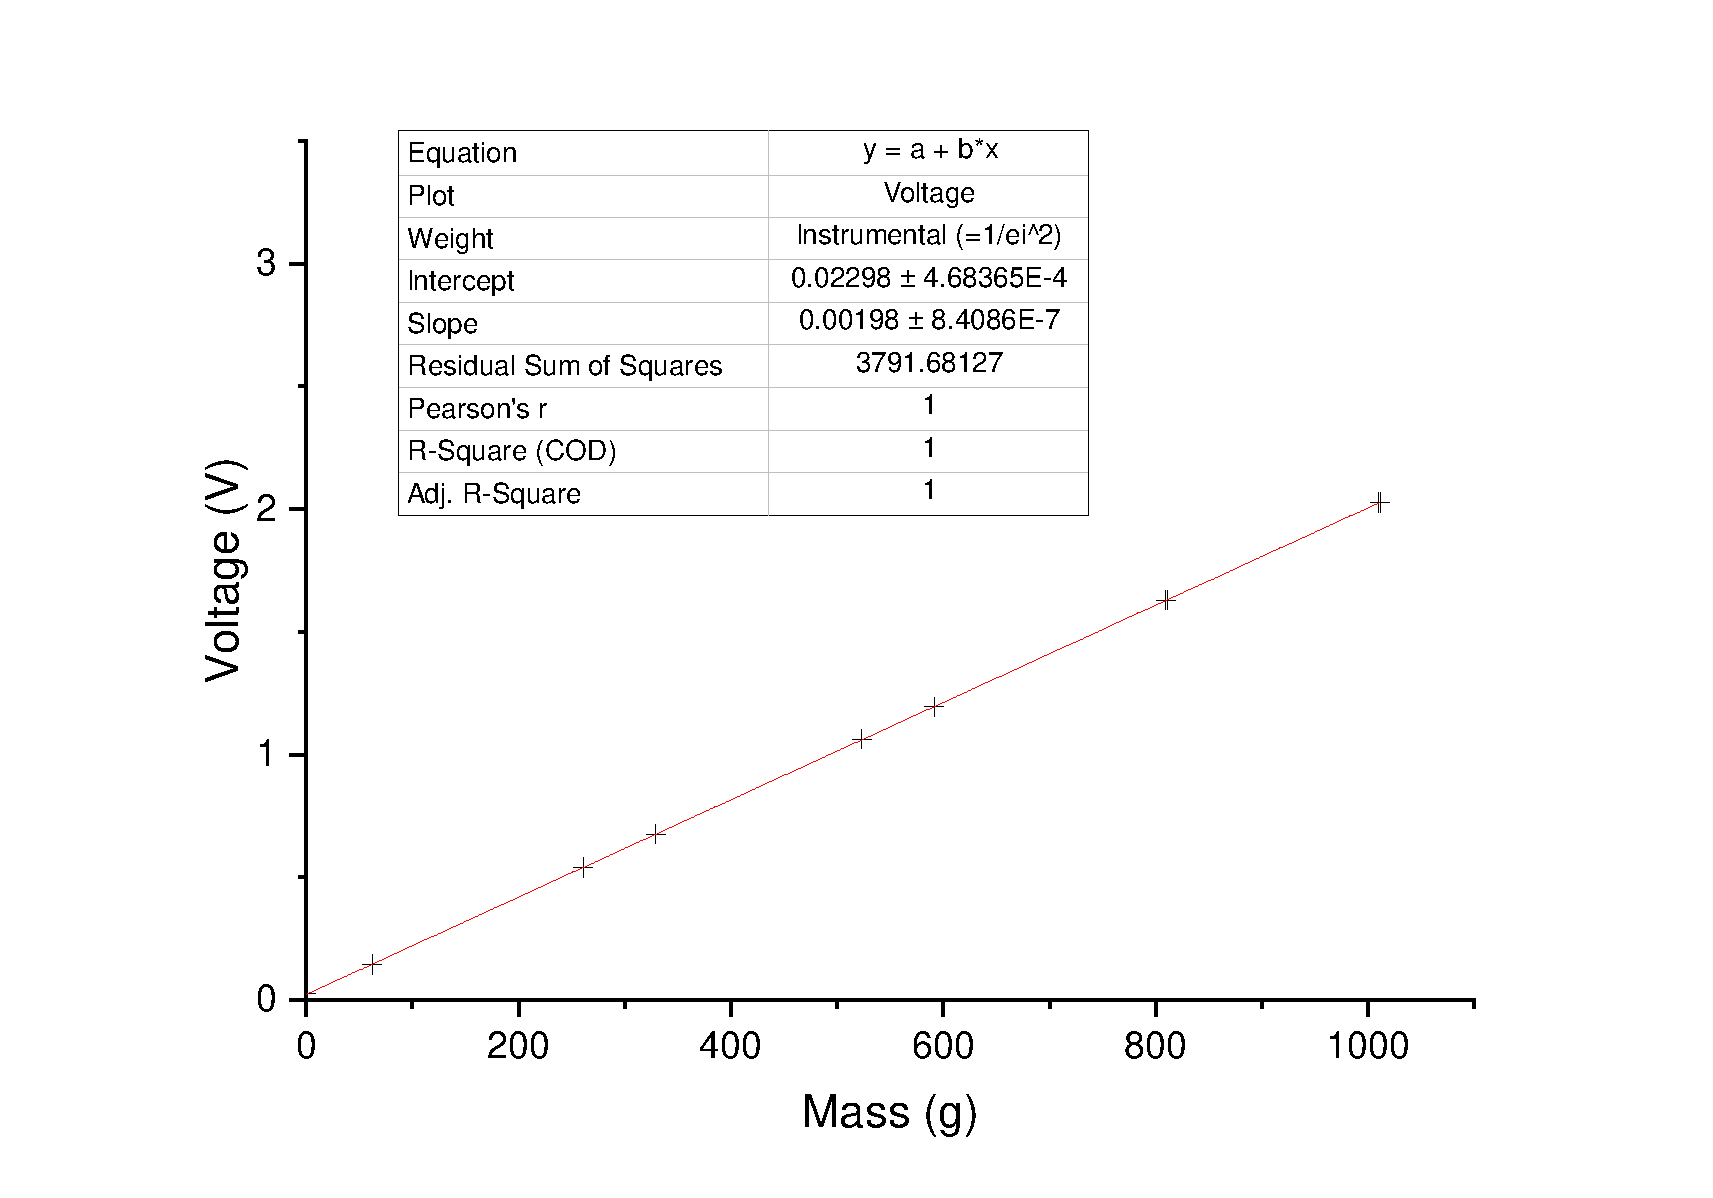
\includegraphics[width=.8\textwidth]{figures/calibr.pdf}
    \caption{Final calibration of or measurement system}
    \label{fig:final_calibration}
\end{figure}
The equation linking the mass to the amplified voltage is : $Voltage = 0.00198.mass+0.02298$, with Voltage in Volts and mass in grams.
\newpage
%----------------------------------------------------------------%
\section{Bibliography}
\bibliography{biblio}
\bibliographystyle{alpha}
\newpage
%----------------------------------------------------------------%
\begin{appendices}
\section{Personal statement on skills}
\subsection{Youwan Mahé}
\paragraph{}
This project is a good manner to evaluate our skills. The two main skills as stated on the school's skill reference document are :
\begin{itemize}
    \item Design or produce technical solution to meet specifications.
    \item Cooperate in a team or in a project mode
\end{itemize}
\subsubsection{Design or produce technical solution to meet specifications}
\paragraph{} 
During this 24 hours project, we had to determine various values for the different building blocks of the printed circuit board. Thanks to the layout of the board, I found it easy to separate the main functions of the circuit. The alimentation, the amplifier, the filter and the Analogue to Digital conversion. Each of the blocks were very basic. The filter for example was a $1^{st}$ order low-pass made with only two components. The ADC was also very simple to use thanks to the $I^2C$ protocol. The study of the overall circuit was made on separate blocks on a first time and on a second time on the whole system. The main metrologic characteristics such as sensitivity or Limit Of Detection (LOD) are determined. The calibration curve shows a good fit without non-linearities. 
\paragraph{}
In addition, every calibration graph meets the specification, such as the weight range (up to 1kg) and limit of detection.
\subsubsection{Cooperate in a team or in a project mode}
The project was a good occasion to work on some soft-skills. Working in duo was easy with my teamate. Each session we had a good workload management. We had tree type of tasks.
\begin{itemize}
    \item Tasks to be done before the session starts. It typically was some calculus or datasheet reading. This could be done at home to save some time for manipulations on the board.
    \item Tasks to be done during the session. It was a list of measurements, soldering, things to ask the teacher during the sessions. Usually we were able to do just what we wanted but nothing more.
    \item Tasks to be done after the lab session. It was usually some data processing and report writing.
\end{itemize}
\paragraph{}
Since Pierre-Louis was better at calculus than myself, he usually took the more mathematical tasks. On the other hand, I produced all the graphs and took care of data processing and logging all the manipulation we did.
\paragraph{}
At the end of this project, I am happy with the result we achieved. In my opinion, we could not do much more in the allowed time, but a lot of work is still to be done in order to go from lab bench to a real product.
\newpage
\subsection{Pierre-Louis Gil}
\paragraph{}
According to the skill sheet, the project can help us improve in the following:
\begin{itemize}
    \item  Designing or producing technical solution to meet specifications
    \item Working in group
\end{itemize}
\subsubsection{Design or produce technical 
solution to meet specifications}
\paragraph{}
During the project, we had to choose correctly the different value of resistor and capacitor as well as which resistor use to achieve a working circuit. Each part of the circuit was tackled independently then the circuit was studied as a whole to ensure that it worked as intended. For example, we used the datasheet of the amplifier to find the value of the gain resistor, but this gain created an offset at the output of the amplifier. The offset being related to another part of the circuit (the strain caused by the platform on the gauge), we also had to consider the previous components to obtain a working circuit which lead us to the appearance of a resistor in the Wheatstone bridge.
\subsubsection{Working in group}
\paragraph{}
During the project, we had two times to work.
\begin{itemize}
    \item At home, where we could work on the theory, read the datasheets and process the result. 
    \item In school where we had the possibility to test as well as designing by testing.
\end{itemize}
The time we had in school was pretty tight so it was difficult to work on every aspect of the circuit. We could have improved it with a little bit more time.
As Youwan was better than me during these school sessions, he handled the majority of the experience we did as well as the welding, I asked for explanation when I needed it to be able to think about these in the future.
My forte being calculus, I did a good part of the maths (resistor and capacitor values, error budget, etc...).
I feel like our team was balanced and that it helped us being efficient.
\paragraph{}
I am happy about the results we produced and it would have been difficult for us to have done more in the limited time we had.
With more we could have studied different parts of the circuit such as the CAN to learn more about it but we could have also be able to improve our design further.
\end{appendices}

\end{document}
